% \documentclass[12pt,doubledspaced,oneside,openright]{qmwphd}
% Final MSc project report using qmwphd.cls
% \usepackage{moreverb} % This defines \verbatiminput.

\documentclass[a4paper,12pt,times]{report}
%PhD Thesis Template for the School of Electronic Engineering and Computer Science, Queen Mary University of London. Stripped from Dan Stowell's PhD.

%BEFORE SUBMISSION DO THESE:
% * deactivate all \includeonly
% * ensure \doneit set to nothing
% * ensure numbering CONTINUOUS from title page on through
% * activate the includes of license, ack, etc
% * check through for question mark errors in render
% * make sure the bibliog doesn't have ugly urls in

%\usepackage{ifdraft}
\usepackage{amsmath}
\usepackage{amsfonts}
\usepackage{amssymb}
%\usepackage{natbib}
%\usepackage{har2nat}
\usepackage{rotating}
\usepackage[breaklinks]{hyperref}
\usepackage{subfig} % apparently subfig is the one to use not subfigure
\usepackage{appendix}
\usepackage{tipa}
\usepackage{clrscode}
\usepackage{setspace}
\usepackage[absolute]{textpos} 

\usepackage{csquotes}
\usepackage[style=authoryear-ibid, backend=bibtex]{biblatex}
\addbibresource{references.bib}

\usepackage{adjustbox}

\usepackage{algorithm}
\usepackage{algorithmic}

\begin{document}

%\setlength{\TPHorizModule}{200mm} 
%\setlength{\TPVertModule}{100mm} 
%\textblockorigin{61mm}{19mm}
	
%%%%% thanks alex mclean for super-useful onscreen reading tip:
%\usepackage[top=0.1in, bottom=0.1in, left=0.3in, right=0.3in, paperwidth=11in, paperheight=7in]{geometry} % activate for ONSCREEN reading shape AT HOME
%\usepackage[top=0.1in, bottom=0.1in, left=0.3in, right=0.3in, paperwidth=11in, paperheight=8.5in]{geometry} % activate for ONSCREEN reading shape AT WORK

\doublespacing{}
\pagenumbering{gobble}
%\frontmatter

% titlepage stuff
\begin{minipage}[t]{0.40\textwidth}
	%\vspace{0.5cm}
	{\large \textbf{School of Electronic\\Engineering and\\Computer Science}}\vspace{16.5cm}\newline
	%{\large School of Electronic\\Engineering and\\Computer Science}\vspace{15.7cm}\newline
	
\includegraphics[scale=0.15]{Logo.png}\vspace{0.5cm}
\end{minipage}
\vline width 2pt
\hspace{0.8cm}
\begin{minipage}[t]{0.60\textwidth}	
	%\vspace{0.5cm}
	{\normalsize MSc Sound and Music Computing}\\
	{\normalsize Project Report 2015}\vspace{5.5cm}\\
	%\begin{doublespace}
	%\title{Hybrid music recommender using content-based and social information}
	\textbf{\Large Hybrid music recommender\\using content-based and\\social information}\newline\\%\vspace{.5cm}\\
	{\large Paulo Esteban Chiliguano Torres}\vspace{7cm}\\%\hspace{0.5cm}\vspace{1.0cm}
		%\textbf{\HUGE Intuitive Gestural\\Interaction with\\Sampled Sounds}\vspace{4.5cm}\\
	%\end{doublespace}
	\flushright
	{\normalsize \today}%\hspace{0.5cm}

\end{minipage}

%\title{Hybrid music recommender using content-based and social information}
%\author{Paulo Esteban Chiliguano Torres \\
%	\\
%	Project Report 2015\\
%	MSc Sound and Music Computing\\
%	\\
%	School of Electronic Engineering and Computer Science\\
%	Queen Mary University of London
%}

%\date{August 2015}


% \author{Paulo Esteban Chiliguano Torres}
% \title{Hybrid music recommender using content-based and social information}
% \qualification{Master of Science} 

%\renewcommand{\abstractname}{Acknowledgements}
%\begin{abstract}
%	Thanks Mum!
%\end{abstract}
\section*{Acknowledgements}
I wish to express my sincere gratitude to Dr. Georgy Fazekas, Lecturer in Digital Media at Queen Mary University of London, for giving me the opportunity to work on this state-of-the-art field and for his guidance and valuable suggestions during the planning and development of this project. I also wish to acknowledge the supplementary assistance provided by Dr. Tony Stockman and Dr. Mathieu Barthet during my time as a student at Queen Mary University of London.
\\
\\
I am particularly grateful with National Government of the Republic of Ecuador for awarding me with a scholarship to study a postgraduate taught degree at a high-quality research university in the United Kingdom of Great Britain and Northern Ireland.
\\
\\
Finally, a special warm thanks goes to my parents, my brothers and Miss Ana Costilla for their support and encouragement throughout my studies.

% \begin{summary}
% \end{summary}
\begin{abstract}

%Background
There is a vast range of Internet resources available today, including songs, albums, playlists or podcasts, that a user cannot discover if there is not a tool to filter the items that the user might consider relevant. Several recommendation techniques has been developed since the internet explosion to achieve this filtering task. In an attempt to recommend relevant song to users, we propose an hybrid recommender that considers real-world users information and high-level representation for audio data. We use a deep learning technique, convolutional deep neural network, to represent the audio data in an abstract level. As our main contribution, we investigate a state-of-the-art technique, estimation of distribution algorithm, to capture the listening behaviour of an individual from the features of the songs that are interesting to the user. The designed hybrid music recommender outperform the predictions compared with a traditional content-based recommender. 
%Aims
%Method

%Results

%Conclusions

\end{abstract}



\tableofcontents
\listoffigures
\listoftables



% Start the main context
% numbering starts from here:
%\mainmatter

\setcounter{page}{1}
\pagenumbering{arabic}
\chapter{Introduction}
Music has accompanied social activities on our daily lives and has influenced the shape of the technology landscape that we have today. Portable media players, mobile device applications or music streaming services enable us the access to a large volume of digital recorded music. This vast range of music tracks might include songs that are relevant or not to a listener, being necessary to develop facilities to bring out appropriate musical pieces to an user.

Recommender systems can be described as engines that guide the users to suitable objects from a large number of options in a particular domain such as books, films or music. The available information of users and items' attributes is analysed and exploited by the recommender systems to produce a list of previously unseen items that each user might find enjoyable. Depending on the analysed data, the design of a recommender can be focused on historical ratings given by users or similarities between the attributes of items that an user already rated.

\section{Motivation}
Due to the available information of relationship between users and items would be sparse, e.g., most part of the users tend to do not give enough ratings, the accuracy of predictions would decrease. Another disadvantage of traditional recommender systems, referred as \textit{cold-start problem}, arises when a new item cannot be recommended until it gets enough ratings, or, equivalently, when a new user does not have any ratings \parencite{melville2010recommender}. In order to alleviate the rating sparsity and cold-start problems, there is the motivation to combine two or more recommendation techniques into hybrid approaches. 

Deep learning is an approach to artificial intelligence for describing raw data as a nested hierarchy of concepts, with each abstract concept defined in terms of simpler representations. For example, deep learning can describe high-level features of an image of a car such as position, colour or brightness of the object, in terms of contours, which are also represented in terms of edges. \parencite{Bengio-et-al-2015-Book}  

Inspired in natural evolution of species, estimation of distribution algorithms (EDAs) \parencite{larranaga2002estimation} are robust techniques developed during the last decade for optimisation in Statistics and Machine Learning fields. EDAs can capture the explicit structure of a population with a probability distribution estimated from the best individuals of that population.

\section{Aims}
We aim to design and implement a hybrid music recommender to mitigate the cold-start problem in a content-based recommendation strategy. The architecture of our hybrid recommender approach combines two fundamental tasks \parencite{recsys2012}: \textit{user modelling} and \textit{information filtering}. Both of these techniques require user-item data to learn user's interest and select items based on their content description, respectively.

In this project, user-item information is obtained from the Taste Profile dataset, which is a complementary subset of the Million Song Dataset \parencite{Bertin-Mahieux2011} and provides real world listeners activity, i.e., play counts of a song. On the other hand, the items to consolidate the music library are obtained by using the unique identifier of each song to fetch its audio data from 7digital.

A convolutional deep neural network (CDNN), which is a deep learning model, is employed to describe the time-frequency content of each audio clip with a n-dimensional vector, whose dimensions represent the probability of a clip to belong to an specific music genre. In this project, we bound the number of music genres to 10.

As a primary contribution of this project, estimation of distribution algorithms (EDAs) are investigated to model user profiles in terms of probabilities of music genres preferences. The algorithms use play count and the content vector of each song in the user's collection to optimise the profile. In addition, each dimension in the content vector is treated as a discrete and continuous variable, for evaluation purposes. To our knowledge, this is the first approach that uses a continuous EDA for user profile modelling in recommender systems.

Each user profile then is compared with the vector representation of an audio clip to compute the similarity value between them. Recommendations for an user are built up by selecting the clips with highest similarity values.

The evaluation of our hybrid music recommender approach is assessed by comparing the results obtained with a traditional content-based recommender.

\section{Thesis outline}

The rest of the report is organised as follows: Chapter~\ref{ch:background} provides an overview in recommender systems. Recommendation process, associated challenges, and related work based on state-of-the-art techniques are discussed. In Chapter~\ref{ch:methodology}, we present our proposed hybrid recommendation approach and describe the stages and algorithms in detail. The experiments and evaluation protocols are to assess the performance of the hybrid recommender presented in Chapter~\ref{ch:experiments}. In Chapter~\ref{ch:results}, we proceed to discuss and analyse the results from the conducted experiments to evaluate the proposed hybrid music recommender. In Chapter~\ref{ch:conclusion}, we present the conclusions and some thoughts for further research.
\chapter{Background}
\label{ch:background}
Recommender systems create opportunities and challenges for industry to understand consumption behaviour of users. In particular, for music industry, the development of recommender systems could improve digital music sales \parencite{ringen_2015}, and also, it could assist the listeners to discover new music through their habits \parencite{1_hypebot.com_2015}. However, when there is no priori information of a new introduced item in a recommender system, known as the \textit{cold-start problem}, popular songs could be favoured in recommendation process instead of items in the \textit{long tail}, i.e., songs that do not have enough ratings. Usually, content-based recommender systems are used to solve the cold-start problem because similarities between items are based on the content without regarding the ratings \parencite{Park200811}. Another solution to address the cold-start problem is to combine recommendation techniques to boost the strengths of each technique in an hybrid architecture. \parencite{melville2010recommender}

In this chapter, we present the importance of online social networks and music services platforms for retrieving user-item information, in conjunction with related work on music recommender systems. Subsequently, a novel approach of an hybrid recommendation model based on estimation of distribution algorithms (EDAs) is introduced and examined.

\section{Online Social Networks}
Social network sites \parencite{JCC4:JCC4393} are defined as: \begin{quote}``Web-based services that allow individuals to (1) construct a public or semi-public profile within a bounded system, (2) articulate a list of other users with whom they share a connection, and (3) view and traverse their list of connections and those made by others within the system.''\end{quote}

During the last decade, online social networks, which are also identified as \textit{social media} platforms, have become the outstanding technologies for retrieving and exchanging multimedia information \parencite{Putzke2014519}. Facebook, Twitter or YouTube, have enabled users to produce and share content on the internet, specially, customers around the world are renovating business models by sharing reviews and comments of products directly to companies. This produced content provides opportunities for research to track consumer's behaviour. \parencite{smith2009social}

In particular, Last.fm\footnote{http://www.last.fm/} is an online radio station that also have the facilities of a social media platform, where a user profile is built up by collecting the music tracks listened on multimedia players through a indexing process called \emph{scrobbling}. This profile may expose music consumption and listening behaviour. \parencite{Putzke2014519}

%\subsection{Last.fm}
\section{Music services platforms}
\label{sec:musicservices}
The Echo Nest\footnote{http://developer.echonest.com/} was a music intelligence company that offered solutions for music discovery and personalisation, dynamic curated sources, audio fingerprinting and interactive music applications. In 2014, The Echo Nest was acquired by Spotify\footnote{https://www.spotify.com/}, which is a commercial music streaming service, where a user can browse and listen music tracks sorted by artists, albums, genres or playlists. 

However, The Echo Nest API is still active for developer community and offers the access to artists, songs, taste profiles and playlists data. Particularly, The Echo Nest API is able to retrieve information limited to a particular music tracks catalogue such as 7digital\footnote{http://developer.7digital.com/}.

Both The Echo Nest and 7digital require to sign up for a free account to get unique keys for OAuth\footnote{http://oauth.net/} authentication in order to retrieve desired information through their respective APIs. As well, free account has limited number of calls, in the case of Echo Nest is limited to 20 request per minute and in the case of 7digital is limited to 4000 request per day.

In this project, we use a The Echo Nest account to get music tracks identifiers for each song in the user-item dataset and we use a 7digital developer account to fetch audio for each music track catalogue identifier. The user-item dataset consist of user - song - play count triplets of the Taste Profile\footnote{http://labrosa.ee.columbia.edu/millionsong/tasteprofile} subset which contains real world listeners activity provided among Echo Nest partners including Last.fm.
%\subsection{7Digital}
%\subsection{APIs}
%The publicly available music related information can be collected from user profiles on social networks using Application Program Interface (API).
%\section{Data Fusion Techniques}
%Combination of multiple sources of information to obtain more relevant parameters is known as data fusion.
%In this study, a cooperative data fusion technique is considered to augment information provided from social network source to content-based system features. \citep{Castanedo2013}

\section{Recommender Systems}
Recommender systems are software or technical facilities to provide items suggestions or predict customer preferences by using prior user information. These systems play an important role in commercial applications to increase sales and convey user satisfaction. In general, recommender systems can be categorised in two major groups: collaborative filtering and content-based filtering \parencite{melville2010recommender}.

\textcite{1242} considers also another methods for music recommendation such as \textit{demographic filtering} and \textit{named context-based}.

\subsection{Collaborative filtering}
In collaborative filtering (CF) \parencite{Yao2015453}, a \emph{m$\times$n} rating matrix (Figure~\ref{fig:useritemmatrix}) represents the relationships between \textit{m} users and \textit{n} items.
\begin{figure}[ht!]
	\centering
	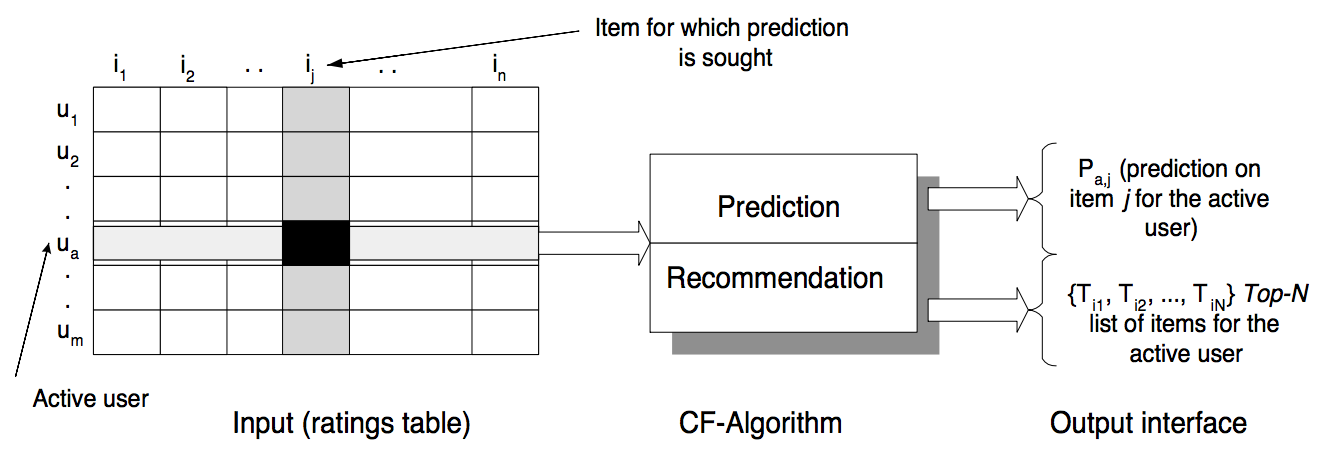
\includegraphics[width=\textwidth]{chapter2/user_item_data.png}
	\caption{Collaborative filtering process \parencite{sarwar2001item}}
	\label{fig:useritemmatrix}
\end{figure}

Recommendations are based on the computed similarities between rows (for users) or columns (for items), hence, CF can be further subdivided in the following neighbourhood models \parencite{Hu2008263}:

\begin{itemize}
	\item \textbf{User based} collaborative filtering, produce a recommendation of a previously unseen item based on similarity between users (Figure~\ref{fig:userbasedcf}).

	\begin{figure}[h!]
		\centering
		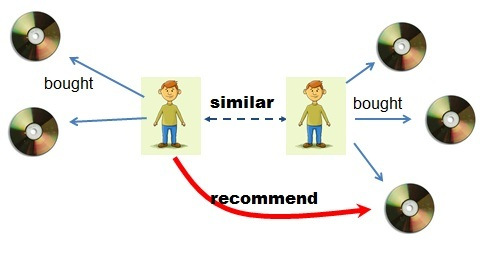
\includegraphics[width=0.5\textwidth]{chapter2/user-user1.jpg}
		\caption{User based collaborative filtering \parencite{1_siddharths_blog_2013}}
		\label{fig:userbasedcf}
	\end{figure}
	
	\item \textbf{Item based} collaborative filtering, produce a recommendation by comparing the similarities between a previously unseen item and the user's items (Figure ~\ref{fig:itembasedcf}).
	
	\begin{figure}[ht!]
		\centering
		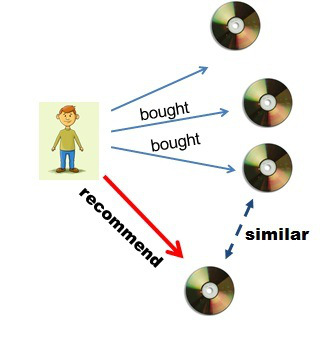
\includegraphics[width=0.4\textwidth]{chapter2/item-item1.jpg}
		\caption{Item based collaborative filtering \parencite{1_siddharths_blog_2013}}
		\label{fig:itembasedcf}
	\end{figure}
	
\end{itemize}

Similarities between a pair of users \emph{a,u} are usually computed with Pearson correlation metric \parencite{sarwar2001item}, given by Equation~\eqref{eq:pearson}:
\begin{equation}
	sim(a,u) =\frac{\sum _{i\in I}(r_{a,i} - \bar{r}_a)(r_{u,i} - \bar{r}_u)}{\sqrt{\sum _{i\in I}(r_{a,i} - \bar{r}_a)^2} \sqrt{\sum _{i\in I}(r_{u,i} - \bar{r}_u)^2}}
	\label{eq:pearson}
\end{equation}
where \emph{I} is the set of items rated by both users, $r_{u,i}$ is the rating given to item \emph{i} by user \emph{u}, and $\bar{r}_u$ is the mean rating given by user \emph{u}. Equivalently, for similarities between a pair of items \emph{i,j}, the correlation is given by Equation~\eqref{eq:pearson2}:
\begin{equation}
sim(i,j) =\frac{\sum _{u\in U}(r_{u,i} - \bar{r}_i)(r_{u,j} - \bar{r}_j)}{\sqrt{\sum _{u\in U}(r_{u,i} - \bar{r}_i)^2} \sqrt{\sum _{u\in U}(r_{u,j} - \bar{r}_j)^2}}
\label{eq:pearson2}
\end{equation}
where \emph{U} is the set of users who have rated both items, $r_{u,i}$ is the rating given to item \emph{i} by user \emph{u}, and $\bar{r}_i$ is the mean rating given to item \emph{i}.

The strength of CF is that the recommendation process is independent of the item features \parencite{Burke2002331}. On the other hand, CF would not be suitable technique when the user-item matrix is sparse. Moreover, CF considers only the most rated items, therefore, ignores the items in the long tail, and it is unable to handle the cold start problem. \parencite{Dai20141760}

\subsubsection{The cold start problem}
Recommendation process in CF might be difficult either for a user or an item with few ratings. \parencite{Burke2002331}

\subsubsection{The long tail phenomenon}
The \textit{long tail} items according to \textcite{Yin2012896} are referred to products with a low volume of sales but they can be more profitable than the popular items if they are recommended to the right consumers.

\subsection{Content-based filtering}
Content based (CB) filtering is based on the analysis of the features that describe the items. The recommendation component consists in matching up the attributes of the items that a user has already rated, usually referred as the \textit{user profile} \parencite{Lops2011}, against the attributes of a previously unseen products to produce a list of \emph{top-N} recommendations. Figure~\ref{fig:cb} shows the architecture of content-based recommendation process.
\begin{figure}[ht!]
	\centering
	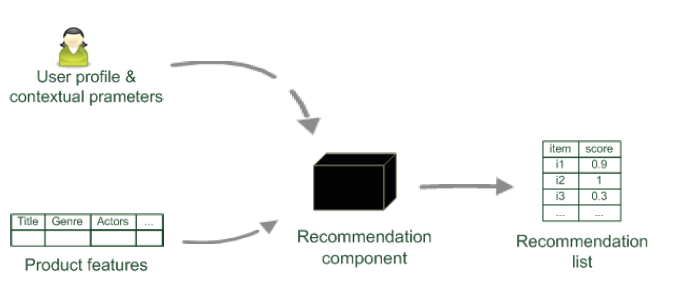
\includegraphics[width=0.8\textwidth]{chapter2/content-based-recommender1.png}
	\caption{Content-based filtering process \parencite{1_blogseagatesoftcom_2015}}
	\label{fig:cb}
\end{figure}

One of the strengths of CB filtering is that recommendation process is entirely based on the attributes of the items, thus, the recommendations produced for each user is independent from the other users information. Also, a CB recommender allows to recommend items that do not have any ratings, therefore, they can diminish the effects of cold-start problem. \parencite{Lops2011}

\subsubsection{Limitations of CB filtering}
One disadvantage of CB filtering is that personal reviews are not considered in the recommendation process, because this technique is limited to explicit representation of items~\parencite{1242}. Moreover, some representations limit the description to certain aspects only~\parencite{Lops2011}.

Another limitation of CB might be the collection of external data due to restricted access, e.g., the Million Song Dataset \parencite{Bertin-Mahieux2011} does not provide audio data due to copyright restrictions\footnote{http://labrosa.ee.columbia.edu/millionsong/pages/can-i-contact-you-privately-get-audio} and some preview clips are not available in the 7digital UK music catalogue. 

In our project, a CB recommender is used as the baseline to show a improved performance in music recommendation. Please refer to Section~\ref{sec:recresults} for more detail.

\subsection{Item Representation}
Items require an accurate description to achieve upstanding results for recommending items to users~\Autocite{1242}. In majority of the content-based filtering systems, item attributes are textual features extracted from web resources.~\parencite{Lops2011}

In our approach, we describe the songs in terms of n-dimensional vectors. Each dimension in the vector represent the probability of the song to belong to a music genre. The probalitity estimation is obtained from a music classifier implemented with a deep learning technique. The song representation process is illustrated in section~\ref{subsec:genre}

\subsection{User Modelling}
``User modeling [sic] is a discipline that deals with both how information about the user can be acquired and used by an automated system.''~\parencite{recsys2012}

Modelling a user profile consists of designing a structure for recording the interests which describe a user. There are several techniques for modelling an user profiles: vector, connexion, ontology and multidimensional representation. \parencite{DBLP:journals/corr/abs-1305-1114}

In our project, we model each user profile through EDAs by minimising a fitness function. The parameters of the fitness function are the rating and similarity values of each song that a user has listened. The user profile is also represented in a n-dimensional vector of probabilities of music genres. This process is illustrated in section~\ref{subsec:profile}

\subsection{Hybrid recommender approaches}
\label{subsec:hybridrecommender}
An hybrid recommender system is developed through the combination of the recommendation techniques mentioned in the previous sections. Usually, hybrid approaches boost the advantages of CF by considering the user's feedback and the advantages of CB by taking into count the item attributes.

According to \textcite{Burke2002331}, there are the following combination methods to accomplish hybridisation:
\begin{itemize}
	\item \textbf{Weighted} method, where a single item recommendation is computed as a linear combination of the recommendation value from each technique involved. The weight assigned to each recommender can be adjusted by considering additional feedback from the user.
	\item \textbf{Switching} method, where the hybrid system uses a criteria depending on the input data to switch between recommendation techniques implemented in the system.
	\item \textbf{Mixed} method, where recommendations from several different types of recommender are presented simultaneously.
	\item \textbf{Feature combination} method, where CF results are treated as additional attributes of a CB filtering recommender.
	\item \textbf{Cascade} method, where one recommender refines the coarse recommendations set given by the first recommender. This method is more efficient than the weighted method, because cascade implementation do not process every item at each stage.
	\item \textbf{Feature augmentation} method, where the rating of an item from one recommender is used as an input feature of another recommendation technique.
	\item \textbf{Meta-level} method, where a model generated for user's interest representation using one recommendation technique is used as the input of another recommender system. The advantage of this method is the performance of the second recommender that uses the compressed representation instead of sparse raw data.
\end{itemize}

The hybrid music recommender approach in this project can be considered as implementation of feature augmentation method and a meta-level method. The general model of our hybrid recommender is explained in detail in Section~\ref{sec:algorithms}.

%is based on a three-way aspect model \citep{Yoshii2008435}. Real item ratings are obtained through Last.fm API and spectral information are represented by convolutional deep belief networks (CDBN) features computed from items' spectrogram \citep{Lee20091096}.

\section{Music Information Retrieval}
Music Information Retrieval (MIR) \parencite{Casey2008668} is a field of research for better human understanding of music data in an effort to reduce the \textit{semantic gap} \parencite{Celma2006} between high-level musical information and low-level audio data. Applications of MIR include artist identification, genre classification and music recommender systems~\parencite{weston2012latent,Yoshii2008435}.

\subsection{Genre classification}
Music classification is one of the main tasks in MIR for clustering audio tracks based on similarities between features of pieces of music. Automatic musical genre classification approach proposed by \textcite{Tzanetakis2002293}, which uses GTZAN genre dataset\footnote{http://marsyas.info/downloads/datasets.html}, has been widely used in the past decade. The GTZAN dataset consists of a total of 1,000 clips, corresponding to 100 examples for each of the 10 music genres: blues, classical, country, disco, hiphop, jazz, metal, pop, reggae and rock. The total duration of each clip is 30 seconds.

Nonetheless, the GTZAN dataset has inaccuracies~\parencite{Sturm20127}, it still provides an useful baseline to compare genre classifiers.

\subsection{Music recommender systems}
\subsubsection{Collaborative retrieval music recommender}
\textcite{weston2012latent} proposed a latent \textit{collaborative retrieval} algorithm using the \textit{Last.fm Dataset - 1K users}\footnote{http://www.dtic.upf.edu/∼ocelma/MusicRecommendationDataset/lastfm-1K.html} dataset. For each (artist, song) tuplet in the dataset, they computed the audio data using 39-dimensional vector corresponding to 13 Mel Frequency Cepstral Coefficients (MFCCs),and the first and the second derivatives. The vectors obtained are used to build up a dictionary using the K-means algorithm. Each audio frame is represented with a vector that contains the number of occurrences of a dictionary vector in the frame. The collaborative retrieval algorithm present outperforming results compared with the Singular Value Decomposition (SVD) and Non-negative Matrix Factorization (NMF) methods used on collaborative filtering recommendation tasks. 

\subsubsection{Hybrid music recommender}
\textcite{Yoshii2008435} proposed a hybrid recommender system considering rating scores collected from Amazon.co.jp and acoustic features derived from the signals of musical pieces corresponding to Japanese CD singles that were ranked in weekly top-20 from April 2000 to December 2005. Acoustic features for each piece are represented as a \textit{bag-of-timbres}, i.e., a set of weights of polyphonic timbres, equivalent to a 13-dimensional MFCC representation. Bags of timbres are computed with a Gaussian Mixture Model, considering the same combination of Gaussians for all the pieces.

A three-way aspect model (see Figure~\ref{fig:threeway}) is used to decompose the joint probability of users \emph{U}, pieces \emph{M} and features \emph{T} into a set of latent genre variables \emph{Z}. It is assumed that user \emph{u} stochastically choose a genre \emph{z} according to their preferences and then the genre \emph{z} stochastically generates a piece of music \emph{m} and an acoustic feature \emph{t}.
\begin{figure}[ht!]
	\centering
	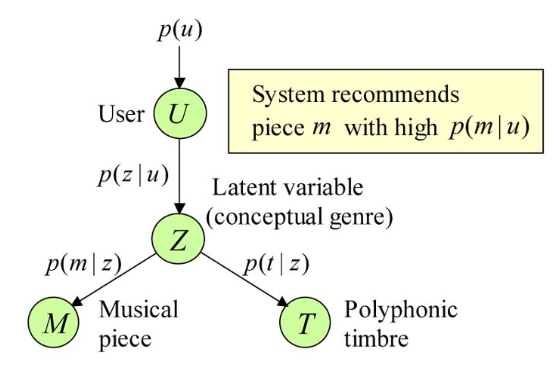
\includegraphics[width=0.5\textwidth]{chapter2/three_way_aspect_model.png}
	\caption{Three-way aspect model~\parencite{Yoshii2008435}}
	\label{fig:threeway}
\end{figure}

The results of the comparative experiments revealed that three-way aspect hybrid method outperformed the CF and CB recommendation techniques in terms of  accuracy considering $\vert T\vert=64$ features and $\vert Z\vert=10$ latent variables.

\section{Deep Learning}
High-level features that help us make sense of an observed data., e.g. genre, mood or release time in a music library could be difficult to compute. Deep learning algorithms allows us to build complex concepts out of simpler concepts \parencite{Bengio-et-al-2015-Book}. Deep learning can solve the difficulty of representing high-level features, e.g., perceived genre in a piece of music, by expressing them in terms of low-level signal features, e.g. spectrum, frequency or pitch.

In MIR, deep learning methods capture the attention of researchers for the following reasons~\parencite{kereliuk15}:
\begin{itemize}
	\item Hierarchical representations of structures in data.
	\item Efficient feature learning and classification algorithms.
	\item Open and publicly available implementations, e.g., \textit{Theano}~\parencite{Bastien-Theano-2012, bergstra+al:2010-scipy} library for Python.
\end{itemize}

These advantages of deep learning methods enable us to learn abstractions from music low-level content in order to reduce the \textit{semantic gap}~\parencite{Celma2006} in MIR. Additionally, feature extraction does not require significant domain knowledge compared to \textit{hand-crafted} engineering. Nonetheless, deep learning implementations require a lot of data.

\subsection{Deep Neural Networks}
A deep neural network (DNN) \parencite{hinton2012deep} is defined as a feed-forward artificial neural network (ANN), or multi-layer perceptron (MLP), with more than one layer of hidden units between the input and the output layer (see Figure~\ref{fig:dnn}).
\begin{figure}[ht!]
	\centering
	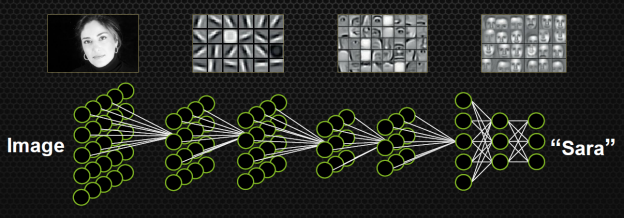
\includegraphics[width=\textwidth]{chapter2/dnn.png}
	\caption{Schematic representation of a deep neural network~\parencite{1_brown_2014}}
	\label{fig:dnn}
\end{figure}

Each hidden unit \emph{j} maps its total input from the layer below $x_j$, given by Equation~\eqref{eq:hiddenunit} 
\begin{equation}
x_j =b_j+\sum_{i}^{}y_iw_{ij}
\label{eq:hiddenunit}
\end{equation}
where $b_j$ is the bias of unit \emph{j}, \emph{i} is an index over units in the
layer below, and $w_{ij}$ is the weight on a connection to unit \emph{j}
from unit \emph{i} in the layer below, to a scalar value $y_j$ that is directed to the layer above. The activation function of hidden units can be hyperbolic tangent, logistic or rectifier linear activation function. For classification, output unit \emph{j} converts its total input $x_j$ into a class probability $p_j$ by using the \textit{softmax} nonlinearity, given by Equation~\eqref{eq:softmax}
\begin{equation}
p_j =\frac{\exp x_j}{\sum_{k}^{}\exp x_k}
\label{eq:softmax}
\end{equation}
where \emph{k} is the number of classes.
\subsubsection{Music Feature Learning}
\textcite{Sigtia20146959} examined and compared DNNs to discover features from the GTZAN dataset and the ISMIR 2004 genre classification dataset\footnote{http://ismir2004.ismir.net/genre\_contest/}, using rectifier linear units (ReLUs) and dropout regularisation. The ReLU activation function is defined as $max(x,0)$. ReLUs provides better convergence without pre-training. Dropout regularisation reduces the problem of overfitting.

First, the GTZAN dataset was divided into four 50/25/25 train, validation, test parts. For each audio clip of the dataset, they calculated the Fast Fourier Transform (FFT) on frames of length 1,024 samples (22,050 kHz sampling rate) with a window overlap of 50\%. Next, they used the magnitude of each FFT frame resulting in a 513 dimensional vector. And then, each feature dimension is normalised to have zero mean and unit standard deviation.

For the deep neural network, the 500 hidden units were trained with stochastic gradient descent (SGD) with a learning rate of 0.01, a patience of 10 and a dropout rate of 0.25.

The system classifies the GTZAN data with an accuracy of 83$\pm$1.1\%, a value of the same order of results obtained with hand-crafted features.

\subsection{Convolutional Deep Neural Networks}
Inspired in the behaviour of animal visual processing system~\parencite{1_deeplearning.net_2015}, a convolutional deep neural network (CDNN)~\parencite{Bengio-et-al-2015-Book, 1_ufldlstanfordedu_2015} is a type of MLP that uses convolution operation instead of matrix multiplication for processing data that has grid-like topology. CDNNs are designed to recognize visual patterns directly from pixel images. In general, the architecture of a CDNN is based on:
\begin{itemize}
	\item \textbf{Sparse connectivity:} the inputs of hidden units in an upper layer \emph{m} are from a subset of units in a lower layer \emph{m$-$1}.
	\item \textbf{Shared weights:} each hidden unit in a layer share the same weight vector and bias. The layer with this parametrisation form a \textit{feature map}.
	%\subitem To preserve the information about the input it is suggested to keeping the total number of activations (number of feature maps times number of pixel positions)
	\item \textbf{Convolutional layers:} A feature map is obtained by convolution of the input image with a linear filter, adding a bias term and then applying a non-linear function. Each convolutional (hidden) layer is composed of multiple feature maps.
	%\subitem The trick is thus to find the right level of “granularity” (i.e. filter shapes) in order to create abstractions at the proper scale, given a particular dataset.
	\item \textbf{Max-pooling:} is a non-linear down-sampling to divide the input image into a set of non-overlapping rectangles and, for each rectangle, the maximum value is returned.
	%Typical values are 2x2 or no max-pooling. Very large input images may warrant 4x4 pooling in the lower-layers.
\end{itemize}

LeNet-5~\parencite{1_lecun_2015} is one model of CDNN designed for recognition of handwritten and machine-printed characters. In Figure~\ref{fig:lenet}, the LeNet model is illustrated. The lower-layers are composed of convolution and max-pooling layers and the upper-layer is a fully-connected MLP. The input to MLP is the set of all features maps at the layer below.
\begin{figure}[ht!]
	\centering
	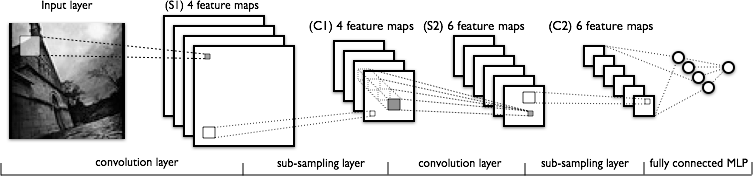
\includegraphics[width=1\textwidth]{chapter2/mylenet.png}
	\caption{Convolutional deep neural network LeNet model \parencite{1_deeplearning.net_2015}}
\label{fig:lenet}
\end{figure}

\subsubsection{Deep content-based music recommendation}
\textcite{NIPS2013_5004} proposed to use a latent factor model for CB recommendation and the implementation of a CDNN to predict the latent factors from music audio. To obtain 50-dimension latent vectors, they used a weighted matrix factorisation (WMF) algorithm on the Taste Profile Subset. Also, they retrieved audio clips for over 99\% of the songs in the dataset from 7digital.com.

To train the CDNN, the latent vectors obtained through the WMF are used as ground truth. The input of the CDNN is a log-compressed mel-spectrogram with 128 components computed from windows of 1,024 samples  and a hop size of 512 samples (sampling rate of 22,050 Hz) for each audio clip. The duration of audio clips is limited to 3 seconds.

They used 10-fold cross validation and obtained an average area under the ROC curve (AUC) of 0.86703 for prediction based on the latent factor vectors, outperforming the bag-of-timbres approach.

\section{Estimation of Distribution Algorithms}
Inspired in natural selection of species, an estimation of distribution algorithm (EDA) \parencite{pelikan2015estimation, Ding2015451, Santana:Bielza:Larrañaga:Lozano:Echegoyen:Mendiburu:Armañanzas:Shakya:2009:JSSOBK:v35i07} is an optimisation technique that estimates a probabilistic model from a sample of promising individuals, which is used to generate a new population and leading to an optimal solution of an objective function, called the \textit{fitness} function, until a termination criteria, e.g., maximisation, minimisation, maximum number of generations, is satisfied. These algorithms were applied to solve complex problems such as load balancing for mobile networks~\parencite{Hejazi15} or software reliability prediction~\parencite{Jin2014113}. In Figure~\ref{fig:eda} we show the general flowchart of an EDA.

\begin{figure}[ht!]
	\centering
	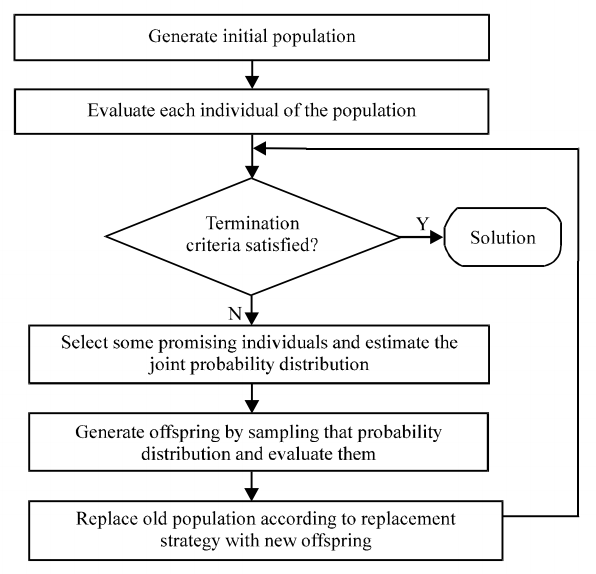
\includegraphics[width=0.5\textwidth]{chapter2/eda.png}
	\caption{Flowchart of estimation of distribution algorithm \parencite{Ding2015451}}
	\label{fig:eda}
\end{figure}

According to~\textcite{pelikan2015estimation}, the main components of an EDA are  a selection operator, a class of probabilistic models for modelling and sampling, and a replacement operator for combining the old population with the offspring. Also, regarding the types of distributions that an EDA are able to capture~\parencite{pelikan2015estimation} can be categorised in four broad groups: 
\begin{itemize}
	\item \textbf{Discrete variables EDAs}, where candidate solutions are represented by fixed-length strings of a finite cardinality.
	\item \textbf{Permutation EDAs}, where candidate solutions are represented by permutations over a given set of elements.
	\item \textbf{Real-valued vectors (continuous) EDAs}, where candidate solutions are mapped from real-valued variables into a discrete domain or the probabilistic model defined on real-valued variables are considered.
	\item \textbf{Genetic programming EDAs}.
\end{itemize}

The advantages of using EDAs include the discovery of problem-specific features or reducing the memory requirements. However, it is time consuming to build explicit probabilistic models.~\parencite{pelikan2015estimation}

In our project, we investigate permutation EDAs and continuous EDAs for user profile modelling.

\subsection{A Hybrid Recommendation Model Based on EDA}
\textcite{Liang2014781} exploited a permutation EDA to model user profiles in an hybrid model for movie recommendation using the MovieLens 1M dataset\footnote{http://grouplens.org/datasets/movielens/}.

A movie, \emph{i}, is described using a vector, $t_i=\{(k_1,w_1),\ldots ,(k_n,w_n)\}$, where the keywords $k_n$ and weights $w_n$ are calculated with term frequency-inverse document frequency (TF-IDF) technique. A user is initially represented by a set,  $S_u=\{(t_1, r_{u,1}),\ldots,(t_i, r_{u,i})\vert r_{u,i}>\bar r_{u}\}$, where, $r_{u,i}$ is the rating of the movie \emph{i} given by user \emph{u}, and $\bar r_{u}$ is a threshold. The keywords in every $S_u$ set are embedded in a new set, $D_u$.

The goal is to learn the user profile, $profile_u=\{(k_1,w_1),\ldots ,(k_n,w_n)\}$, by minimisation of the fitness function, defined by Equation~\eqref{eq:fitness}
\begin{equation}
fitness(profile_u) =\sum_{i\in S_u}\log(r_{u,i}\times sim(profile_u,t_i))
\label{eq:fitness}
\end{equation}
where $sim(profile_u,t_i)$ is computed by the cosine similarity coefficient, defined by Equation~\eqref{eq:cossim}
\begin{equation}
sim(profile_u, t_i)=cos(profile_u, t_i) =\frac{profile_u\cdot t_i}{\Vert profile_u\Vert\times\Vert t_i\Vert}
\label{eq:cossim}
\end{equation}

The pseudocode of EDA implemented by \textcite{Liang2014781} is delineated by Algorithm~\ref{alg:hybrideda}, where MAXGEN is the maximum number of generations.
\begin{algorithm}[ht!]
	\caption{Calculate $profile_u$}
	\begin{algorithmic} 
		\REQUIRE set $D_u$, weights $w_{n,i}$
		\REQUIRE population size $N$, MAXGEN
		%\ENSURE $y = x^n$
		\STATE Random selection of keywords $k_n$ from $D_u$
		\STATE Assign a weight $w_{n,i}$ to each $k_n$ to build a set~$K_u$ of size~$N$
		\STATE Assign a probability $c_{n,i}=1/N$ to each $(k_n,w_{n,i})$
		\STATE Generate initial population of $profile_u$ by Monte Carlo method
		\WHILE{$generation <$ MAXGEN}
		\STATE Compute each $fitness(profile_u)$
		\STATE Rank individuals by their fitness value
		\STATE Select top $M < N$ individuals
		\STATE Update $c_{n,i}$ by counting the occurrences of $(k_n,w_{n,i})$ in the $M$ individuals profiles
		\STATE Generate $profile_u$ by random sampling according to updated $c_{n,i}$
		\ENDWHILE
		\RETURN $profile_u$
	\end{algorithmic}
	\label{alg:hybrideda}
\end{algorithm}

To recommend a new movie, \emph{j}, to a user, the similarity between the user profile, $u_i$, and the movie vector, $t_j$, is calculated using Pearson correlation coefficient, defined by Equation~\eqref{eq:wpearson}:
\begin{equation}
sim(u_i,t_j) =\frac{\sum _{c\in I_i \cap I_j}^{ } (w_{i,c} - \bar{w}_i)(w_{j,c} - \bar{w}_j)}{\sqrt{\sum _{c\in I_u \cap I_j}^{ }(w_{i,c} - \bar{w}_i)^2} \sqrt{\sum _{c\in I_u \cap I_j}^{ }(w_{j,c} - \bar{w}_j)^2}}
\label{eq:wpearson}
\end{equation}
where, $c\in I_i \cap I_j$ are the keywords in common between the user profile and the new movie vector, $w_{i,c}$ and $w_{j,c}$ are the weights of keyword \emph{c} in the user profile and movie vector, $\bar{w}_i$ is the mean weight of user profile and $\bar{w}_j$ is the mean weight of movie vector.

In our approach, we use the algorithm proposed by~\textcite{Liang2014781} to model user profiles but considering probability values of music genres instead of weight values of keywords. The adapted algorithm is explained in subsection~\ref{subsec:profile}.

\subsection{Continuous Univariate Marginal Distribution Algorithm}

\textcite{gallagher2007bayesian} presented the continuous univariate marginal distribution algorithm ($UMDA_c^G$) as an extension of a discrete variable EDA. The general pseudocode of the $UMDA_c^G$ is delineated in Algorithm~\ref{alg:umda}, where $x_i\in \textbf{x}$ represent the \emph{i} parameter of \textbf{\emph{x}} individual solution.

\begin{algorithm}[ht!]
	\caption{Framework for $UMDA_c^G$}
	\begin{algorithmic} 
		\REQUIRE population size $M$
		\REQUIRE selection parameter $\tau$
		%\ENSURE $y = x^n$
		\STATE $t \leftarrow 0$
		\STATE Generate $M$ individuals at random
		\WHILE{$t <$ stopping criteria}
		\STATE $M_{sel}\leftarrow M\cdot\tau$
		\STATE Select $M_{sel}$ individuals 
		\STATE $\mu_{i,t}\leftarrow\frac{1}{M_{sel}}\sum_{j=1}^{M_{sel}}x_i^j$
		\STATE $\sigma_{i,t}^2\leftarrow\frac{1}{M_{sel}-1}\sum_{j=1}^{M_{sel}}(x_i^j-\mu_{i,t})^2$ 
		\STATE $p_t({x_{i}}\vert \mu_{i,t},\sigma_{i,t}^2)\leftarrow\frac{1}{\sqrt{2\pi}\sigma_{i,t}}\exp(-\frac{1}{2}(\frac{x_i-\mu_{i,t}}{\sigma_{i,t}})^2)$
		\STATE Sample $M$ individuals from $p_t({x_{i}}\vert \mu_{i,t},\sigma_{i,t}^2)$
		\STATE $t\leftarrow t+1$
		\ENDWHILE
	\end{algorithmic}
	\label{alg:umda}
\end{algorithm}

To our knowledge, our hybrid recommender design is the first work to consider a continuous EDA for user profile modelling in a recommender system. The implementation of the continuous EDA is explained in subsection~\ref{subsec:profile}.

\section{Summary}
In this chapter, previous work on recommender systems has been reviewed and novelty techniques to representing acoustical features and to model user profiles has been presented. The next steps are to collect the dataset by crawling online social information, to extract the acoustical features of a collection of songs to represent them as n-dimensional vectors, to model the user profiles by using EDAs, and therefore, to return a list of song recommendations.
\chapter{Methodology}
\label{ch:methodology}
The methodology used to develop our hybrid music recommender consists of four main stages. First, the collection of real world user-item data corresponding to the play counts of specific songs and the fetching of audio clips of the unique identified songs in the dataset. Secondly, the implementation of the CDNN to represent the audio clips in terms of music genre probabilities as n-dimensional vectors. Next, permutation EDA and a continuous EDA are investigated to model user profiles based on the rated songs above a threshold. Finally, the process of top-N recommendation for the baseline and the hybrid recommender is described.

Every stage of our hybrid recommender is entirely developed in Python 2.7\footnote{https://www.python.org/download/releases/2.7/}, although, they are implemented in different platforms, e.g., OS X (v10.10.4) for the most part of the implementation, Ubuntu (14.04 LTS installed on VirtualBox 5.0.0) for intermediate time-frequency representation and CentOS (Linux release 7.1.1503) for the data preprocessing and CDNN implementation.

\section{Data collection}
The Million Song Dataset \parencite{Bertin-Mahieux2011} is a collection of audio features and metadata for a million contemporary popular music tracks which provides ground truth for evaluation research in MIR. This collection is also complemented by the Taste Profie subset which provides 48,373,586 triplets, each of them consist of anonymised user ID, Echo Nest song ID and play count. We choose this dataset because it is publicly available data and it contains enough data for user modelling and recommender evaluation.

\subsection{Taste Profile subset cleaning}
Due to potential mismatches\footnote{http://labrosa.ee.columbia.edu/millionsong/blog/12-2-12-fixing-matching-errors} between song ID and  track ID on the Echo Nest database, it is required to filter out the wrong matches in the Taste Profile subset. The cleaning process is illustrated in Figure~\ref{fig:taste_profile} 
\begin{figure}[ht!]
	\centering
	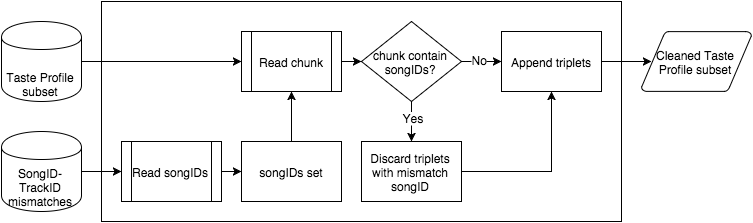
\includegraphics[width=0.9\textwidth]{chapter3/taste_profile.png}
	\caption{Diagram of the cleaning process of the Taste Profile subset}
	\label{fig:taste_profile}
\end{figure}
%Please see figure ~\ref{fig:JobInformationDialog} 

A script is implemented to discard the triplets that contain the song identifiers from the mismatches text file. First, we load the file to read each line of it to obtain song identifier. The identifiers are stored as elements of a set object to construct a collection of unique elements. Next, due to the size of the Taste Profile subset (about 3 GB, uncompressed), we load the dataset by chunks of 20,000 triplets in a \textit{pandas}\footnote{http://pandas.pydata.org/} dataframe to clean each chunk by discarding the triplets that contains the song identifiers in the set object of the previous step. The cleaning process takes around 2.47 minutes and we obtain 45,795,100 triplets. 

In addition to the cleaning process, we reduce significantly the size of the dataset for experimental purposes. We only consider users with more than 1,000 played songs and select the identifiers of 1,500 most played songs. This additional process takes around 3.23 minutes and we obtain 65,327 triplets. The triplets are stored in a cPickle\footnote{https://docs.python.org/2/library/pickle.html\#module-cPickle} data stream (2.8 MB).

%count resulting number of triplets
%At this stage, similarities between users is calculated to form a neighbourhood and predict user rating based on combination of the ratings of selected users in the neighbourhood.

\subsection{Fetching audio data}
First, for each element of the list of 1,500 songs identifiers obtained in the previous step is used to retrieve the associated Echo Nest track ID through a script using the \emph{get\_tracks} method from the \textit{Pyechonest}\footnote{http://echonest.github.io/pyechonest/} package which allow us to acquire track ID and preview URL for each song ID through Echo Nest API. The reason behind this is 7digital API uses Echo Nest track ID instead of song ID to retrieve any data from its catalogue. If the track information of a song is not available, the script skips to retrieve the Echo Nest information of the next song ID. At this point, it is useful to check if the provided 7digital API keys, a preview URL, and the country parameter, e.g., 'GB' to access to UK catalogue, work in the \textit{OAuth 1.0 Signature Reference Implementation}\footnote{http://7digital.github.io/oauth-reference-page/}.

Next, for each preview URL, we can create a GET request using \textit{python-oauth2}\footnote{https://github.com/jasonrubenstein/python\_oauth2} package, because it allows us to assign the nonce, the timestamp, the signature method and the country parameters. The request is converted to a URL to be opened with \textit{urlopen} function from the \textit{urllib2}\footnote{https://docs.python.org/2/library/urllib2.html} module, to download a MP3 file (44.1 kHz, 128 kbps, stereo) of 30 to 60 seconds of duration in a song repository.

Considering the Echo Nest API and 7digital API limited number of requests (see Section~\ref{sec:musicservices}), the process of fetching data from 1,500 song IDs takes at least 8 hours, resulting in a total of 640 MP3 files.

Additionally, the script accumulates the Echo Nest song identifier, track ID, artist name, song title and the 7digital preview audio URL for each downloaded track in a text file only if the audio clip is available for download. The generated text file is used for the preprocessing of the cleaned taste profile dataset in subsection~\ref{subsec:rating}. The flowchart of the script is shown in Figure~\ref{fig:fetchaudio}
\begin{figure}[ht!]
	\centering
	\includegraphics[width=0.9\textwidth]{chapter3/fetch_audio.png}
	\caption{Flowchart of the fetching audio process}
	\label{fig:fetchaudio}
\end{figure}

%include number of tracks available

%Classifier creates a model for each user based on the acoustic features of the tracks that user has liked.
\subsection{Intermediate time-frequency representation for audio signals}
\label{subsec:spectrogram}
Intermediate audio representation instead of waveform (time-domain) representation is required to feed a CDNN according to \textcite{NIPS2013_5004}. The flowchart to obtain the time-frequency representation from raw audio content of the song repository assembled in the previous section is shown in Figure~\ref{fig:timefrequency}.
\begin{figure}[ht!]
	\centering
	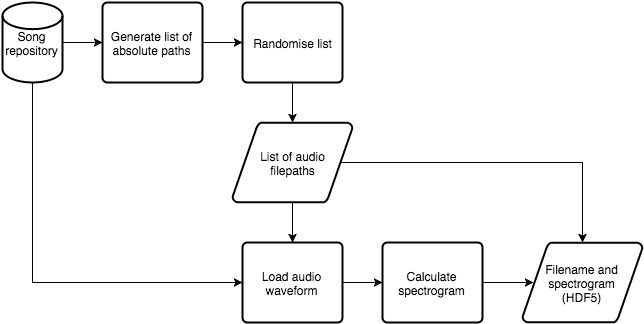
\includegraphics[width=0.7\textwidth]{chapter3/time_frequency.png}
	\caption{Flowchart for time-frequency representation process}
	\label{fig:timefrequency}
\end{figure}

First, a list of absolute paths corresponding to the songs in the repository is generated. The sequence of paths in the list is modified by random shuffling. This new sequence of absolute paths is saved in a text file.

Second, for every path in the text file of randomised absolute paths, a fragment equivalent to 3 seconds of the associated audio clip is loaded at a sampling rate of 22,050 Hz and converted to mono channel. For every fragment, a mel-scaled power spectrogram with 128 bands is computed from windows of 1,024 samples with a hop size of 512 samples, resulting in a spectrogram of 130 frames with 128 components. Hence, the spectrogram is converted to logarithmic scale in dB using peak power as reference. The functions \textit{load}, \textit{feature.melspectrogram} and \textit{logamplitude}, correspondingly to load an audio clip, spectrogram computation and logarithmic conversion, from the LibROSA\footnote{https://bmcfee.github.io/librosa/index.html} package are used.

To handle audio with LibROSA functions, it is recommended to use the Samplerate\footnote{https://pypi.python.org/pypi/scikits.samplerate/} package for efficient resampling. In our project, we considered to use the SoX\footnote{http://sox.sourceforge.net/} cross-platform without success due to operating system restrictions. Alternatively, we use the FFmpeg\footnote{https://www.ffmpeg.org/} cross-platform and \textit{libmp3lame0}\footnote{http://packages.ubuntu.com/precise/libmp3lame0} packages for efficient resampling.

Finally, we store the absolute path and the log-mel-spectrogram values of the 640 songs in a HDF5\footnote{https://www.hdfgroup.org/HDF5/} data file.

In the particular case for the time-frequency representation of each audio clip in the GTZAN dataset, we generate a list of the genre associated to each audio fragment that represent the target values (ground truth). This procedure for the GTZAN dataset is repeated for 9 times, considering the rest of 3-seconds fragments in each audio clip of the dataset for training, validation and testing of the CDNN (see Section~\ref{subsec:genre})

The time elapsed to obtain the time-frequency representation of the clips in the GTZAN dataset with the procedure described above is about 55 seconds, generating a HDF5 file (66.9 MB). Because of the number of MP3 files in the song repository is less than the number of files of the GTZAN dataset, the process is faster and the size of the HDF5 file is smaller (42.8 MB).

\section{Data preprocessing}
In order to obtain suitable representations for users' interest in the taste profile dataset and for songs' spectrograms, it is necessary an additional process of the data.
\subsection{Rating from implicit user feedback}
\label{subsec:rating}
First, the text file of the downloaded MP3 metadata (see subsection~\ref{subsec:spectrogram}) is used to retain the triplets, from the cleaned taste profile subset, that contain the song IDs of the available audio clips. A reduced taste profile dataset with 4,685 triplets is obtained, corresponding to information of 53 users.

The reduced taste profile dataset represent the user listening habits as implicit feedback, i.e., play counts of songs, it is necessary to normalise the listening habits as explicit feedback, i.e., range of values $[1\ldots5]$ that indicate how much a user likes a song. Normalisation of play counts is computed with the complementary cumulative distribution of play counts of a user, following the procedure given by \textcite{1242}. Songs in the top 80 - 100\% of the distribution get a rating of 5, songs in the 60 - 80\% range get a 4, songs in the 40 - 60\% range get a 3, songs in the 20 - 40\% get a 2 and songs in the 0 - 20\% range get a rating of 1. An exception for this allocation of ratings comes out when the coefficient of variation, given by Equation~\eqref{eq:cv}:
\begin{equation}
CV=\frac{\sigma}{\mu}
\label{eq:cv}
\end{equation}
where, $\sigma$ is the standard deviation and $\mu$ is the mean of the play counts of a user, is less or equal than $0.5$. In that case, every song gets a rating of 3.

\subsection{Standardise time-frequency representation}
\label{subsec:normalised}
The logarithmic mel-scaled power spectrograms obtained in subsection~\ref{subsec:spectrogram} are normalised to have zero mean and unit variance in each frequency band, using the \textit{fit} and \textit{transform} methods of the \textit{StandardScaler} class from the Scikit-learn~\parencite{scikit-learn} package, as a common requirement of several machine learning classifiers.

Additionally, the GTZAN normalised spectrograms dataset is split in 3 subsets: 500 spectrograms for training, 250 spectrograms for validation and 250 spectrograms for testing. Each spectrogram is saved as a tuple \textit{(spectrogram, tag)} in a cPickle file, where tag is the number of the music genre: 0 for blues, 1 for classical, 2 for country, 3 for disco, 4 for hiphop, 5 for jazz, 6 for metal, 7 for pop, 8 for reggae and 9 for rock.

\section{Algorithms}
\label{sec:algorithms}
The hybrid music recommender approach in this project can be considered as implementation of feature augmentation method and a meta-level method presented in subsection~\ref{subsec:hybridrecommender}. First, user profiles are generated using the rating matrix and the song vector representation. Next, the model generated is the input of a CB recommender to produce \emph{top-N} song recommendations. The general model of our hybrid recommender is shown in Figure~\ref{fig:generalhybrid}
\begin{figure}[ht!]
	\centering
	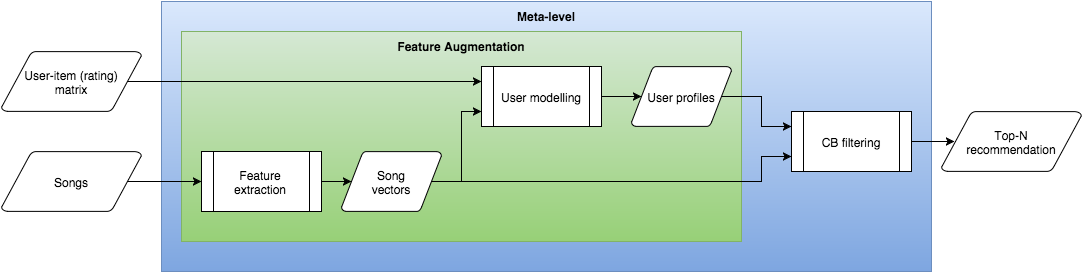
\includegraphics[width=\textwidth]{chapter3/General_model_hybrid_recommender.png}
	\caption{Diagram of the hybrid music recommender}
	\label{fig:generalhybrid}
\end{figure}

\subsection{Probability of music genre representation}
\label{subsec:genre}
To represent an audio file in a 10-dimensional vector, whose dimensions correspond to the 10 music genres specified in the GTZAN dataset, a CDNN is implemented using Theano library. For intensive computation processes, such as convolution, the implementation on equipment with Graphical Processing Unit (GPU) acceleration is recommended. In this project, a CentOS (Linux release 7.1.1503) server with a Tesla K40c\footnote{http://www.nvidia.com/object/tesla-servers.html} GPU is exploited.

The scripts for logistic regression, multilayer perceptron and deep convolutional network designed for character recognition of MNIST\footnote{http://www.iro.umontreal.ca/~lisa/deep/data/mnist/mnist.pkl.gz} dataset, available on~\textcite{1_deeplearning.net_2015} is adapted to our purpose of music genre classification. ReLU and dropout functions are defined in the deep convolutional network script.

%Deep belief network is a probabilistic model that has one observed layer and several hidden layers.
\subsubsection{CDNN architecture}
\begin{figure}[ht!]
	\centering
	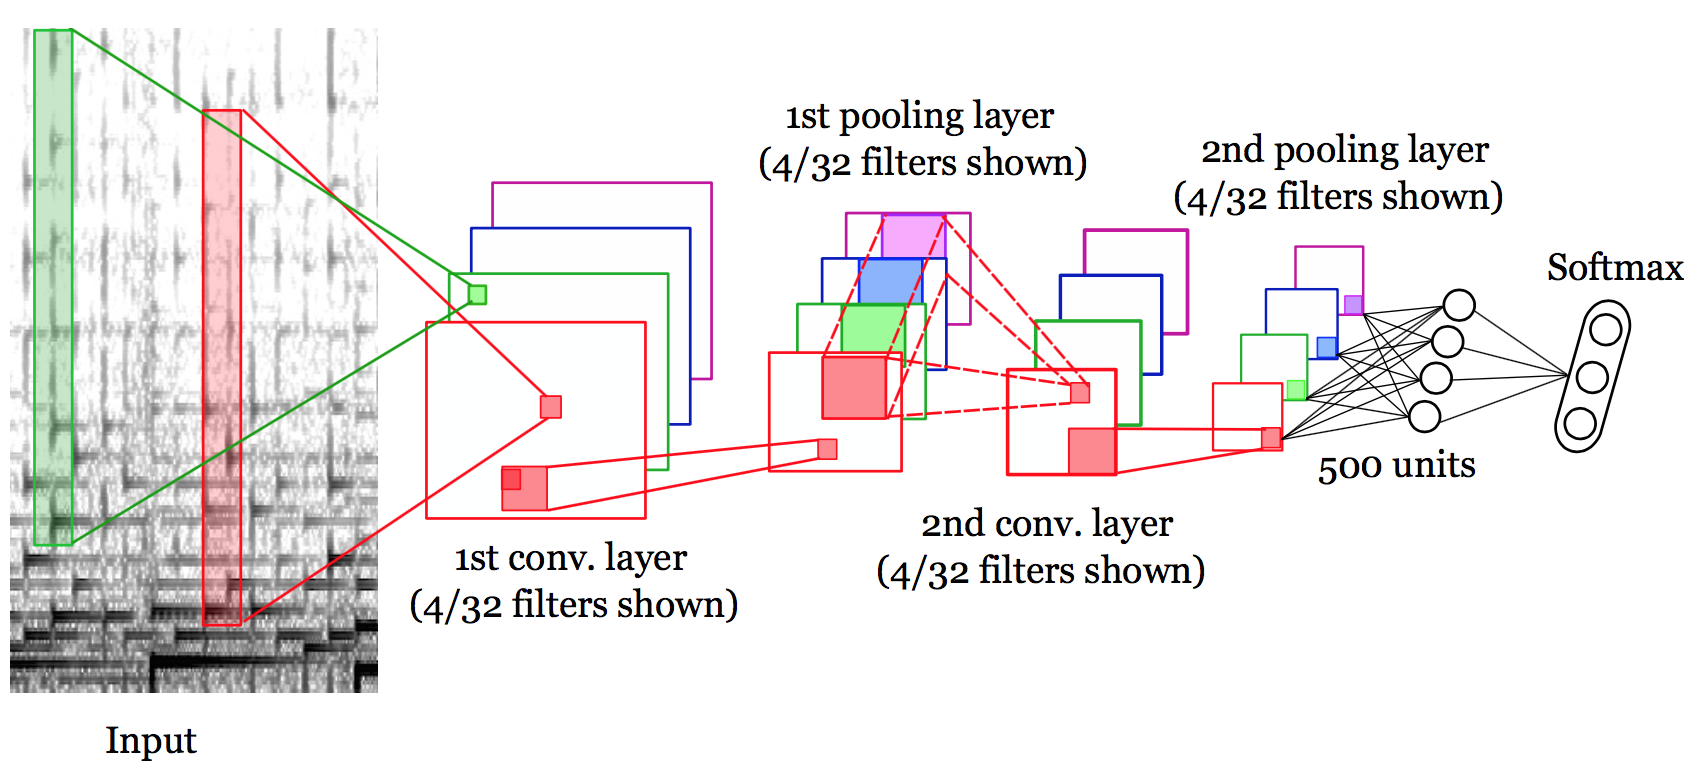
\includegraphics[width=\textwidth]{chapter3/CDNN.png}
	\caption{Diagram of CDNN for music genre classification~\parencite{kereliuk15}}
	\label{fig:cdnn}
\end{figure}
A similar architecture of a CDNN for music genre classification~\parencite{kereliuk15} is recreated in our project. A batch size of 20 and a dropout rate of 0.20 for the convolutional layer units are considered.

Initially, the reshape of the 2-dimension normalised spectrograms (130 frames$\times$128 frequency bands) obtained in subsection~\ref{subsec:normalised} to a 4-dimension tensor, compatible with the input of the first convolutional layer (batch size$\times$1$\times$130$\times$128), is required.

The first convolutional layer consists of 32 filters, each one with a size of 8 frames, with a max-pooling downsampling of 4, to reduce the size of the spectrogram along the time axis. The size of the resulting spectrogram is 30$\times$128 and the output of this first convolutional layer is a 4-dimension tensor with a size of 20$\times$32$\times$30$\times$128.

The second convolutional layer consists of 32 filters, each one with a size of 8 frames, with a max-pooling downsampling of 4, to reduce the size of the spectrogram obtained in the first layer. The size of the new spectrogram is 5$\times$128 and the output of this second convolutional layer is a 4-dimension tensor with a size of 20$\times$32$\times$5$\times$128.

Following the convolution process, the reshape of the 4-dimensional tensor of the output of the second convolutional layer is required to feed the fully connected MLP. The MLP consists of 500 ReLUs.

Finally, the classification of music genre is accomplished with logistic regression layer of the 500 output values from the MLP. This output layer consists of 10 units with softmax activation function (see Equation~\eqref{eq:softmax}).

\subsubsection{Learning parameters}
The weights and biases of the units of the CDNN are the parameters
to be modelled by SGD to minimise a cost function. The cost function is the negative log likelihood of the prediction in the output layer given the target values, i.e., music genre ground truth.

The CDNN for training, validation and testing is run for 200 epochs, each epoch equivalent to 50 iterations. The number of iterations corresponds to the ratio between the number of spectrograms (1,000 for GTZAN dataset) and the batch size.

According to \textcite{bengio2012practical}, the patience value is the minimum number of training examples. In our project, the patience value is set at 1,000.

In our testing, after 9 trials in the CDNN, we obtain a best classification error of 38.8 \% using the spectrograms corresponding to the GTZAN dataset (see Table~\ref{table:genre}). The weights and biases for this best classification error are saved in a cPickle file to be applied as initial parameters of the CDNN for vector representation.

\subsubsection{Vector representation}
The script of CDNN is adapted to produce the vector representation of the spectrograms. This CDNN uses the weights and biases learnt in genre classification process as initial parameters.

A 10-dimension vector is produced by the softmax output layer. Each dimension corresponds to a music genre and each value represents the probability of a song to belong to a specific music genre, given the normalised spectrogram at the input layer.

\subsection{User profile modelling}
\label{subsec:profile}
To model user profiles from the triplets in the normalised taste profile dataset, we adapt the permutation EDA (see algorithm~\ref{alg:hybrideda} on page ~\pageref{alg:hybrideda}) and the continuous EDA (see algorithm~\ref{alg:umda} on page ~\pageref{alg:umda}). For both EDAs, we consider the following:
\begin{itemize}
	\item User representation $S_u=\{(t_1, r_{u,1}),\ldots,(t_i, r_{u,i})\vert r_{u,i}>\bar r_{u}\}$.
	\item Rating threshold $\bar r_{u}\}=2$, assuming that a user does not like songs with ratings of 1 and 2 out of 5.
	\item The stopping criteria is the maximum number of generations limited to 250.
\end{itemize}


\subsubsection{Modelling with Permutation EDA}
In the case of permutation EDA, the genre tags (0 for blues, 1 for classical, 2 for country, 3 for disco, 4 for hiphop, 5 for jazz, 6 for metal, 7 for pop, 8 for reggae and 9 for rock) are considered as the keywords $k_n$ in the set $D_u$ and the weights $w_{n,i}$ are 50 evenly spaced samples over the interval $[0.1, 0.9]$, thus, the size of the set $K_u$ is $N=500$ and the initial probability is $c_{n,i}=1/500$.

The population size is equal to $u=53$, that is the number of users in the normalised taste profile dataset. Instead of using the Monte Carlo method to generate the initial population of $profile_u$, 10 tuples $(k_n,w_{n,i})$ from $K_u$ are random sampled for each user. The number of top individuals $M$ is a half of the total of users. The process of sampling new individuals is preserved. The adapted permutation EDA for user modelling is illustrated in Algorithm~\ref{alg:permutationeda}:

\begin{algorithm}[ht!]
	\caption{Calculate $profile_u$ for users in taste profile}
	\begin{algorithmic} 
		\REQUIRE set $D_u$, weights $w_{n,i}$
		\REQUIRE population size $u$, MAXGEN
		\REQUIRE $M = Round(u/2)$
		%\ENSURE $y = x^n$
		%\STATE Random selection of keywords $k_n$ from $D_u$
		\STATE Assign a weight $w_{n,i}$ to each $k_n$ to build a set~$K_u$ of size~$N$
		\STATE Assign a probability $c_{n,i}=1/N$ to each $(k_n,w_{n,i})$
		\STATE Generate initial population of $profile_u$
		\WHILE{$generation <$ MAXGEN}
		\STATE Compute each $fitness(profile_u)$
		\STATE Rank individuals by their fitness value
		\STATE Select top $M < N$ individuals
		\STATE Update $c_{n,i}$ by counting the occurrences of $(k_n,w_{n,i})$ in the $M$ individuals profiles
		\STATE Generate $profile_u$ by random sampling according to updated $c_{n,i}$
		\STATE $generation\leftarrow generation+1$
		\ENDWHILE
		\RETURN $profile_u$
	\end{algorithmic}
	\label{alg:permutationeda}
\end{algorithm}

The time elapsed for modelling user profiles with the permutation EDA is approximately 7.82 seconds.

\subsubsection{Modelling with $UMDA_c^G$}
The $UMDA_c^G$ algorithm is adapted to select the top $M_{sel}$ individuals by using the fitness function (Equation~\eqref{eq:fitness} on page~\pageref{eq:fitness}) exploited by the permutation EDA. The population size is $M=53$ users, the selection parameter is $\tau=0.5$. $x_i$ represent the probability value of the music genre dimension, \emph{i}, in the $profile_u$ vector.

In each generation, \emph{t}, the mean value $\mu_{i,t}$ and the variance $\sigma_{i,t}^2$ is computed for every dimension, $i$, along the $M_{sel}$ individuals vectors. For each dimension, i.e., music genre, the normal distribution is calculated with its corresponding mean value and variance, to estimate the  individuals vectors of the next generation.
\begin{algorithm}[ht!]
	\caption{Framework for $UMDA_c^G$ to model users}
	\begin{algorithmic} 
		\REQUIRE population size $M$
		\REQUIRE selection parameter $\tau$
		\STATE Generate $M$ individuals at random
		\STATE $M_{sel}\leftarrow M\cdot\tau$
		\STATE $t \leftarrow 0$
		\WHILE{$t <$ MAXGEN}
		\STATE Compute each $fitness(profile_u)$
		\STATE Rank individuals by their fitness value
		\STATE Select top $M_{sel}$ individuals 
		\STATE $\mu_{i,t}\leftarrow\frac{1}{M_{sel}}\sum_{j=1}^{M_{sel}}x_i^j$
		\STATE $\sigma_{i,t}^2\leftarrow\frac{1}{M_{sel}-1}\sum_{j=1}^{M_{sel}}(x_i^j-\mu_{i,t})^2$ 
		\STATE $p_t({x_{i}}\vert \mu_{i,t},\sigma_{i,t}^2)\leftarrow\frac{1}{\sqrt{2\pi}\sigma_{i,t}}\exp(-\frac{1}{2}(\frac{x_i-\mu_{i,t}}{\sigma_{i,t}})^2)$
		\STATE Sample $M$ individuals from $p_t({x_{i}}\vert \mu_{i,t},\sigma_{i,t}^2)$
		\STATE $t\leftarrow t+1$
		\ENDWHILE
	\end{algorithmic}
	\label{alg:umda2}
\end{algorithm}
The time elapsed for modelling user profiles with the continuous EDA is approximately 4.20 seconds.
\subsection{Top-N songs recommendation}
The final stage of the recommender systems implemented is to generate a list of song recommendations according to the similarity values computed with Equation~\eqref{eq:wpearson} (see page~\pageref{eq:wpearson}).
\subsubsection{Top-N recommendations in CB baseline}
The list of recommendations in a CB recommender is given by the similarities between the items that a user has already rated and the new items. It is assumed the user has not seen before the new items.

First, the similarity matrix between every item in the training set is computed. Only the $k=30$ most similar items are kept for each item. Next, for each song that a user rated above the threshold (rating $>$ 2), the $k$ neighbours are retrieved as a list of candidate items. The list is normalised to have a maximum value of 1. The lists of candidates are appended. For the repeated candidates, the similarity values are summed up. The $N$ candidates with higher similarity values are recommended to a user.

\subsubsection{Top-N recommendations in hybrid music recommender}
In our hybrid music model (see Figure~\ref{fig:generalhybrid} on page~\pageref{fig:generalhybrid}), the content based filtering computes the similarity between a user interest profile and a each song vector in the test set. The songs are ranked in descending order and the first $N$ songs of this ranking are recommended.

In our project, we experiment with different values for N, obtaining the best results with the hybrid music recommender based on permutation EDA for all the experiments. Refer to Section~\ref{sec:recresults} for detailed results of evaluation.

\section{Summary}
In this chapter, we presented the collection and preprocessing of the taste profile subset to model the user profiles with EDAs. As well, we presented the procedure of time-frequency representation of the audio content to feed a CDNN in order to obtain a 10-dimension vector representation corresponding to the probability of a song to belong to a music genre. Also, we presented the adapted architecture of the CDNN and the EDAs for hybrid recommendation. In the following chapter, we introduce the evaluation method and experiments to evaluate our hybrid recommender approach.
\chapter{Experiments}
\label{ch:experiments}
In order to evaluate the performance of a recommender system, there are several scenarios to be considered depending on the structure of the dataset and the prediction accuracy. It is therefore necessary to determine a suitable experiment for the evaluation of our proposed hybrid music recommender that employs a rating matrix and vector representation of songs as inputs to produce \textit{top-N} song recommendations.

In addition, the performance of our hybrid approaches is compared with a pure content-based recommender algorithm.

%\section{Experiment aims}
%deviation between the actual and predicted ratings is measured 
%the prediction ratings are compared with a model-based collaborative filtering.

\section{Evaluation for recommender systems}

\subsection{Types of experiments}
The scenarios for experiments requires to define an hypothesis, controlling variables and generalization of the results. Three types of experiments \parencite{export:115396} can be used to compare and evaluate recommender algorithms:
\begin{itemize}
\item \textbf{Offline experiments:} where recorded historic data of users' ratings are used to simulate online users behaviour. The aim of this type of experiment is to refine approaches before testing with real users. On the other hand, results may have biases due to distribution of users.
\item \textbf{User studies:} where test subjects interact with the recommendation system and its behaviour is recorded giving a large sets of quantitative measurements. One disadvantage of this type of experiment is to recruit subjects that represent the population of the users of the real recommendation system.
\item \textbf{Online evaluation:} where the designer of the recommender application expect to influence the users' behaviour. Usually, this type of evaluation are run after extensive offline studies.
\end{itemize}

\subsection{Evaluation strategies}
On the other hand, evaluation of recommender systems can be classified \parencite{1242} in:
\begin{itemize}
\item \textbf{System-centric} process has been extensively exploited in CF systems. The accuracy of recommendations is based exclusively on users' dataset and is evaluated through predictive accuracy, decision based and rank based metrics.
\item \textbf{Network-centric} process examines other components of the recommendation system, such as diversity of recommendations, and they are measured as a complement of the metrics of system-centric evaluation.
\item \textbf{User-centric:} The perceived quality and usefulness of recommendations for the users are measured via provided feedback.
\end{itemize}

\subsection{Decision based metrics}
Our hybrid recommender produces a list of songs for each user, hence, it is necessary to evaluate the recommendation with a metrics derived from \textit{confusion matrix} that reflects the categorisation of test items as true positives (TP), false positives (FP), true negatives (TN) and false negatives (FN). In this project we consider the following metrics \parencite{1242}:
\begin{itemize}
	\item \textbf{Precision} is the ratio of correct positive predictions.
	\begin{equation}
	Precision = \frac{TP} {TP+FP}\label{eq:1}
	\end{equation}
	\item \textbf{Recall} is the ratio of positive instances predicted as positive.
	\begin{equation}
	Recall = \frac{TP} {TP+FN}\label{eq:2}
	\end{equation}
	\item \textbf{F1 measure}, is the harmonic relation of precision and recall.
	\begin{equation}
	Recall = \frac{2 \times Precision \times Recall} {Precision+Recall}\label{eq:3}
	\end{equation}
	\item \textbf{Accuracy}, is the ratio of correct predictions.
	\begin{equation}
	Recall = \frac{TP+TN} {TP+FP+TN+FN}\label{eq:4}
	\end{equation}
\end{itemize}


%Text \eqref{eq:1}


%Text \eqref{eq:2}


\section{Evaluation method}
The hybrid music recommender system proposed in this project is evaluated through an offline experiment and the results are presented with decision based metrics described in the previous section.

\subsection{Training set and test set}
The normalised taste profile dataset (refer to subsection~\ref{subsec:rating}) is split in a training and a test set. For each user in the dataset, a random sample corresponding to 20 \% of the total number of ratings is assigned to the test set, and the rest 80 \% is assigned to the training set. The split process is iterated for 10 times, resulting in a total of 10 training and 10 test sets.

\subsection{Top-N evaluation}
For each song in the user test set, we look up if the song is included or not in the list of top-N recommendations.

If the test song is in the top-N recommendation and if the rating of the test song is above the threshold (rating $>$ 2), we count as a true positive, otherwise is counted as a false positive.

If the test song is not in the top-N recommendation and if the rating of the test song is above the threshold, we count as a false negative, otherwise is counted as a true positive.

%\subsection{Evaluation measures}
%Because the dataset does not include explicit ratings, hence, the number of plays of tracks are considered as users' behaviours,


\section{Results}

\begin{itemize}
\item 20\% of song ratings is the test set, the other 80\% is the training set, for each user. The number of users evaluated is 53.
\item For each song in the  test set, we look up if the song is included or not
in the produced top-N recommendations.
%\item Examples of classification results are shown below:
\end{itemize}

\begin{center}
\resizebox*{1.0\columnwidth}{!}{

	\begin{tabular}{c| c| c| c| c} % centered columns (4 columns)
		\hline\hline %inserts double horizontal lines
		Recommender & Precision & Recall & F1 & Accuracy \\ [0.5ex] % inserts table
		%heading
		\hline % inserts single horizontal line
		Content-based (baseline) & 0.275 $\pm$ 0.087 & 0.010 $\pm$ 0.003 & 0.020 $\pm$ 0.007 & 0.681 $\pm$ 0.008 \\ % inserting body of the table
		Hybrid (discrete EDA) & \textbf{0.391 $\pm$ 0.182} & \textbf{0.013 $\pm$ 0.007} & \textbf{0.025 $\pm$ 0.013} & \textbf{0.685 $\pm$ 0.009} \\
		Hybrid (continuous UMDA) & 0.318 $\pm$ 0.142 & 0.011 $\pm$ 0.005 & 0.021 $\pm$ 0.011 & 0.683 $\pm$ 0.009 \\ [1ex] % [1ex] adds vertical space
		\hline %inserts single line
	\end{tabular}

}
\end{center}
%\begin{center}
%\begin{tabular}{c@{ }c@{ }c@{ }c@{ }c@{ }c@{ }c}
%bananas &
%\resizebox*{0.12\columnwidth}{!}{\includegraphics{images/fruit/bananas2.eps}} &
%\resizebox*{0.12\columnwidth}{!}{\includegraphics{images/fruit/bananas2.eps}} &
%\resizebox*{0.12\columnwidth}{!}{\includegraphics{images/fruit/bananas2.eps}} &
%\resizebox*{0.12\columnwidth}{!}{\includegraphics{images/fruit/bananas2.eps}} &
%\resizebox*{0.12\columnwidth}{!}{\includegraphics{images/fruit/plums2.eps}} &
%\resizebox*{0.12\columnwidth}{!}{\includegraphics{images/fruit/bananas2.eps}} \\
%plums &
%\resizebox*{0.12\columnwidth}{!}{\includegraphics{images/fruit/plums2.eps}} &
%\resizebox*{0.12\columnwidth}{!}{\includegraphics{images/fruit/bananas2.eps}} &
%\resizebox*{0.12\columnwidth}{!}{\includegraphics{images/fruit/plums2.eps}} &
%\resizebox*{0.12\columnwidth}{!}{\includegraphics{images/fruit/plums2.eps}} &
%\resizebox*{0.12\columnwidth}{!}{\includegraphics{images/fruit/plums2.eps}} &
%\resizebox*{0.12\columnwidth}{!}{\includegraphics{images/fruit/plums2.eps}} \\
%\end{tabular}
%\end{center}

\chapter{Conclusion}
\label{ch:conclusion}
The whole aim of our project has been the design and the implementation of an hybrid music recommender in order to mitigate the cold-start problem in content-based recommender systems. We investigated several types of hybridisation in recommender systems to choose a suitable architecture (shown in~\ref{fig:generalhybrid}) for the available datasets. To represent real world users and raw waveforms, we decided to investigate and implement state-of-the-art techniques.

Despite of the success in computer vision field, we found in our project that convolutional deep neural networks achieve similar results to long-established music genre classifier approaches in music information retrieval field.

Due to the natural selection concept associated to estimation of distribution algorithms, we investigated and considered these optimisation techniques for modelling users' listening behaviour in terms of probabilities of music genres from the songs in they listened.

On the other hand, we found that a limited number of genres for song representation lead us to coarse predictions according to decision-based metrics.

\section{Future work}

For the future, we have the intention to enhance our hybrid music recommender considering a wide range of music genres or latent vectors for item representation. We shall work on investigating several configurations of convolutional deep neural networks and different types of deep learning techniques, particularly, unsupervised learning approaches, for a better high-level representation of audio waveforms. In addition, we will continue investigating the fascinating estimation of distribution algorithms, considering another fitness functions to optimise, to model user profiles in recommender systems. Finally, we also consider the evaluation of hybrid recommender with an online experiment.

%\bibliographystyle{agsm}
\addcontentsline{toc}{chapter}{References}
\printbibliography[title=References]

%\backmatter

\end{document}